\documentclass[a4]{article}
\usepackage[utf8]{inputenc}
\usepackage[brazil]{babel}
\usepackage{url}
\usepackage{tabularx}
\usepackage{palatino}
\usepackage{hyperref}
\usepackage{graphicx}
\usepackage{float}
\usepackage[margin=2cm]{geometry}

\title{\textbf{Lista 1 de IPN0007 - Redes Neurais na Engenharia Nuclear}}
\author{
    \textbf{Aluno:} Luís Felipe de Melo  \\
    \textbf{Número USP:} 9297961
    }
\date{}
\begin{document}
\maketitle

\section*{Exercício 1}

Vida Artificial (VA) é um conceito que descreve os estudos que procuram modelos computacionais para problemas biológicos e tentam criar soluções baseadas na biologia para problemas de engenharia. As técnicas de VA são inspiradas em como os organismos vivos funcionam.

A Inteligência Artificial (IA) também se inspira na vida para suas técnicas. No entanto, o foco é na inteligência, propriamente dita, procurando técnicas de raciocínio, por exemplo. O principal modelo seguido na IA é o cérebro.

\section*{Exercício 2}

As Redes Neurais Artificiais (RNA) são sistemas de aprendizado de máquina baseados nos neurônios humanos. Assim como seu equivalente biológico, as redes neurais são compostas de unidades de processamento simples que são combinadas em camadas.

Como mencionado acima, sua origem é a neurociência, que estuda o sistema nervoso humano. O objetivo primário era de modelar redes neurais reais, mas com a evolução dos estudos da área de IA, elas vêm sendo aplicadas para resolver problemas do mundo real.

\section*{Exercício 3}

As RNA são diferentes dos sistemas computacionais pois elas fazem um raciocínio a partir dos dados que recebem, aprendendo certos comportamentos e adquirindo capacidade de generalização. Os sistemas computacionais executam programas, não sendo capaz de entender a organização de um conjunto de dados e se adaptar a ele.

\section*{Exercício 4}

O primeiro modelo de neurônio artificial é "Neurônio de McCulloch-Pitts", desenvolvido em 1943. Ele recebe um vetor de valores de entrada $ x $ e o multiplica a um vetor de pesos $ w $. Feito isso, ele soma cada um dos valores resultantes e os passa por uma função de ativação, gerando a saída. O esquema segue abaixo:

\begin{figure}[H]
	\centering
	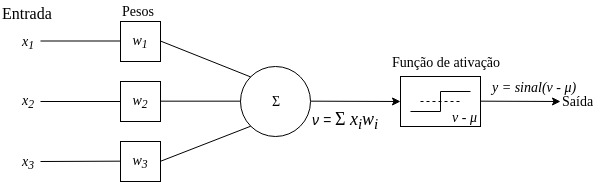
\includegraphics[width=0.8\linewidth]{neuronio.jpg}
	\caption{O neurônio de McCullough-Pitts}
\end{figure}

\section*{Exercício 5}

Uma Função de Ativação é uma função que recebe um valor $ \ni $, que é o produto escalar dos vetores de entrada $ x $ e de pesos $ w $, e devolve um valor que mostra o quanto o neurônio está ativado, dado o valor de entrada. Funções de ativação que costumam ser usadas são a função sinal, linear, sigmoide, entre outras.
 
\section*{Exercício 6}

Os dendritos são partes de um neurônio (prolongamentos) que são responsáveis por receber estímulos nervosos do ambiente e repassá-los para o corpo da célula. Cada neurônio possui vários dendritos. 

\section*{Exercício 7}

O axônio é a parte de um neurônio que é responsável por transmitir os estímulos nervosos do corpo da célula para um local mais distante, como um músculo ou até outro neurônio. Cada neurônio possui apenas um axônio.

\section*{Exercício 8}

As RNA se aplicam a problemas que possuem modelagem difícil, ou que não possuem uma teoria para modelagem, ou que precisam de generalização. São exemplos de problemas assim: processamento de linguagem natural, reconhecimento de padrões (como escrita e imagens), entre outros.

\section*{Exercício 9}

Um "algoritmo de aprendizado" é um algoritmo que aprende a partir de dados de entrada, um certo \textit{feedback} sobre eles (que pode vir junto com os dados ou em uma validação, por exemplo), além de ter a habilidade de aprender com seus erros. Esses algoritmos conseguem fazer previsões sobre os dados, fazendo uma generalização que não é feita por sistemas de computação normais.

\section*{Exercício 10}



\end{document}
